In this chapter we will specify with detail the system requirements and particular features to be implemented. The requirements
will be divided in two major sections.\\
\indent First we will describe what tasks the Back-end of the system should perform in order to provide
all the data and tools for supporting the system Front-end. Then with the end user in mind we will define the tool requirements from
the user point of view. For aggregator that is part of the Front-end no requirements will be specified since this component will only bridge
requests from the Front-end and the Back-end or will eventually fetch data directly from the database.

\section{Social Networks Prioritization}
Before diving into the requirements we first will review our \glspl{osn} preferences regarding information extraction and the
interest we have in analyzing this specific networks.\\
\indent First we want to analyze \textbf{Facebook} because it is the more general purpose network, the more popular and the more used
thus allowing us to derive more interesting conclusions since the resultant graphs will be more realistic having a more concrete social structure
representation. Second we want to analyze \textbf{LinkedIn} because it also widely used and the only one that specifically
focus on professional worldwide networking, generating different kinds of graphs and understand how companies and professionals
are interacting online. Analyzing LinkedIn may also introduce an interesting analysis that is merging information from Facebook and
analyzing friendship networks within professional networks.\\
\indent Having two networks embedded in the system proves that we can analyze social networks in general since we have more
then one and with different purposes, but since the system is designed to simply accommodate new networks simply adding
a new extraction module should the major part of the work to integrate a new \glspl{osn}, this said we could eventually
also implement some extra modules to the remaining \glspl{osn} listed in Chapter 3.

\section{Back-end}
As seen is Figure \ref{img:architectureprop}, our Back-end is essentially composed by essentially two parts: \textbf{web crawlers/extraction modules} and the \textbf{data miner} (that is also an extraction manager), we will write the requirements for each one of the components.

\subsection{Web crawlers}
Each web crawler (or extraction module) must fulfill common requirements that are listed below \footnote{These requirements are agnostic to the \glspl{osn} context}:
\begin{enumerate}
    \item Web crawlers should be able to login with an user account (an \textit{entry point});
    \item Web crawlers should be able to navigate trough the pages of a given \glspl{osn};
    \item Web crawlers must be capable of performing "human" interactions such as click and scroll;
    \item Web crawlers should be able to output a pre defined (agreed and formally defined in the next section) data schema, covering eventual
    exceptions due to privacy limitations;
    \item Web crawlers must be able to perform user extraction with second order depth, from the user entry point perspective (this means that we want to extract user's friends and friends of friends information);
    \item Extraction modules should provide a global extraction method where extraction parameters can be passed from the outside reducing or amplifying scope of extraction as specified from the outside (e.g. under given circumstances we may only need to extract the friends' list or the basic information like name, city and birth date);
    \item Extraction modules must be available to the data miner trough a web API in order to allow remote and distributed extraction. The web API must wrap all the different supported \glspl{osn} being each one accessible trough a different path within the same web api. The API specification may be consulted in the Apendix \textbf{XXX}, page \textbf{XXX}.
\end{enumerate}

\subsection{Data miner}
Below are the data miner requirements \footnote{Again, these requirements are agnostic to the \glspl{osn} context}:

\begin{itemize}
    \item Orchestration of extraction processes scattered trough various hosts: one should be able to define a list of hosts and the number of extraction processes that each host should handle;
    \item Chunk an entry point (that is a set of user identifiers within the \glspl{osn}) in order to delegate different users to different hosts;
    \item Call the extraction endpoints according to the \glspl{osn} from where we need to extract data;
    \item Receive extraction data and normalize the fields that may need some treatment giving as result a normalized data structure;
    \item Store normalized data in the database.
\end{itemize}

\subsection{Extraction pipeline}
Being listed above the requirements for each component we will now draw the specification of what is the expected workflow for data extraction, we will design the pipeline for extraction, that tries to reflect with maximum detail the listed requirements.

\begin{figure}[h!]
\begin{center}
  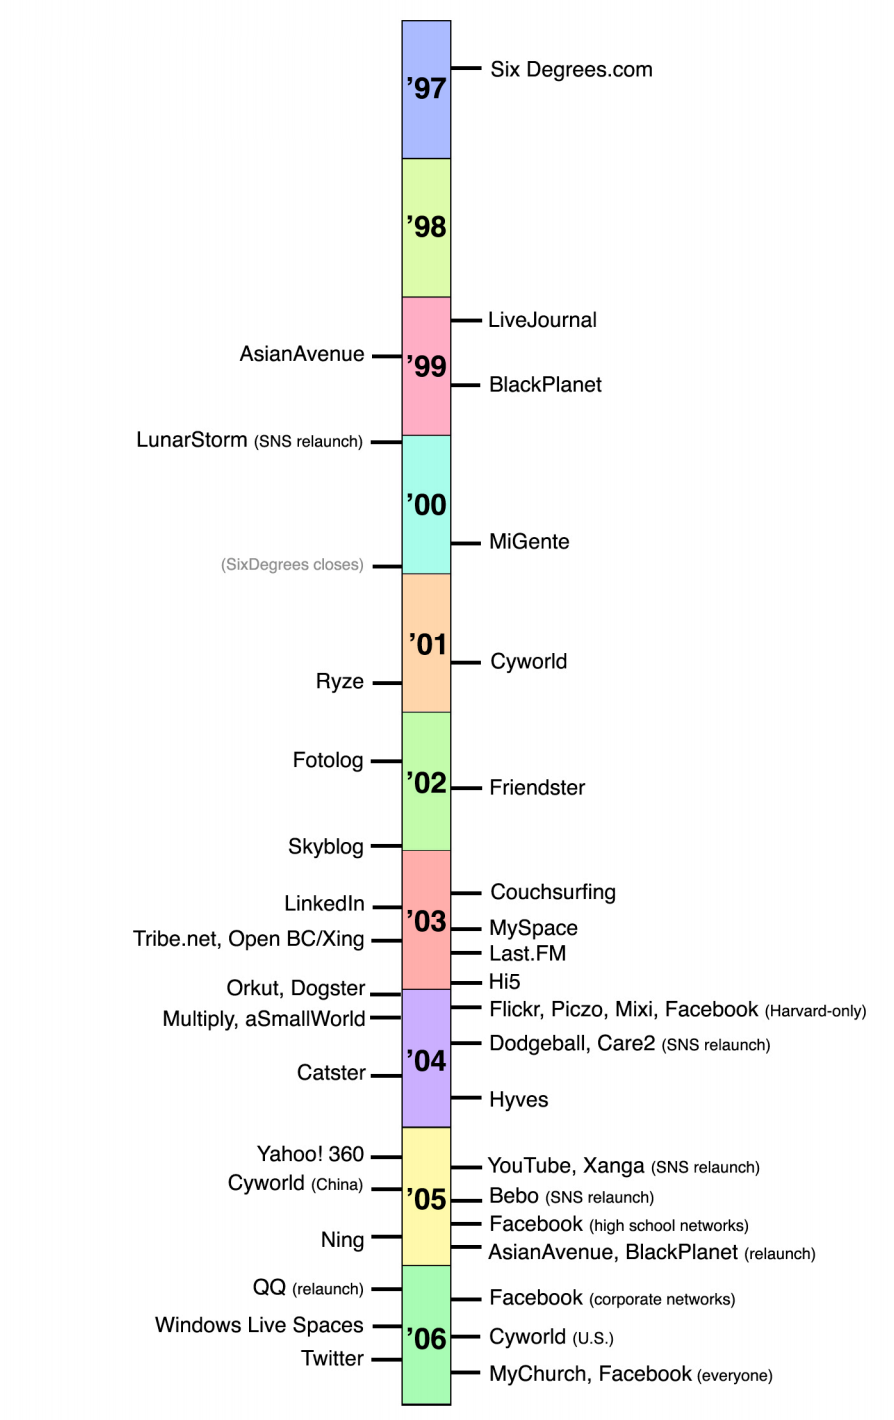
\includegraphics[width=0.7\textwidth]{img/timeline.png}
\end{center}
\caption{\label{img:extpipeline} Extraction pipeline design.}
\end{figure}

As we can see from Figure XXX ... ... ...








\clearpage

\subsection*{Facebook data structure}
\textbf{JSON schema}
\begin{verbatim}
    {
        "livesIn": {
            "id": {string},
            "description": {string}
        },
        "life_events": {
            {string}: [{string}]
        },
        "birthDate": {string},
        "likes": {
            {string}: {string}
        },
        "friends": [{string}],
        "relationships": {
            "civil_status": {
                "id": {string},
                "description": {string}
            },
            "family_members": [
                { "id": {string}, "relationship": {string} }
            ]
        },
        "from": {
            "id": {string},
            "description": {string}
        },
        "name": {string},,
        "gender": {string},
        "age": {number},
        "posts": [
            {
                "timestamp": {string},
                "description": {string},
                "author": {string},
                "reactions": {
                    "likes": {number},
                    "laugh": {number},
                    "sad": {number},
                    "angry": {number},
                    "surprise": {number}
                },
                "comments": {number},
                "shares": {number}
            }
        ]
    }
\end{verbatim}

\subsection*{Linkedin data structure}
\textbf{JSON schema}
\begin{verbatim}
    {
        "id": {string},
        "name": {string},
        "headline": {string},
        "from": {string},
        "summary": {string},
        "experience": [
            {
                "company": {string},
                "position": {string},
                "duration": {
                    "count": {number},
                    "unit": {string},
                    "from": {string},
                    "to": {string}"
                }
            }
        ],
        "education": [
            {
                "institution": {string},
                "course": {string},
                "startYear": 2015,
                "endYear": 2017
            }
        ],
        "skills": {
            {string}: 7
        },
        "languages": {
            {string}: {string}
        },
        "projects": [
            {
                "name": {string},
                "date": {string},
                "description": {string}
            }
        ],
        "groups": [
            {string}
        ],
        "following": [
            {string}
        ],
        "connections": [
            {string}
        ]
    }
\end{verbatim}



\section{Front-end}
Visual requirements, interaction etc. etc.
goals...
all ideas discharge here
